\documentclass[11pt]{article}
\usepackage[utf8]{inputenc}	% Para caracteres en español
\usepackage{amsmath,amsthm,amsfonts,amssymb,amscd}
\usepackage{multirow,booktabs}
\usepackage[table]{xcolor}
\usepackage{fullpage}
\usepackage{lastpage}
\usepackage{enumitem}
\usepackage{fancyhdr}
\usepackage{mathrsfs}
\usepackage{wrapfig}
\usepackage{setspace}
\usepackage{hyperref}
\usepackage{calc}
\usepackage{multicol}
\usepackage{cancel}
\usepackage[retainorgcmds]{IEEEtrantools}
\usepackage[margin=3cm]{geometry}
\usepackage{amsmath}
\newlength{\tabcont}
\setlength{\parindent}{0.0in}
\setlength{\parskip}{0.05in}
\usepackage{empheq}
\usepackage{framed}
\usepackage[most]{tcolorbox}
\usepackage{xcolor}
\colorlet{shadecolor}{orange!15}
\parindent 0in
\parskip 12pt
\geometry{margin=1in, headsep=0.25in}
\theoremstyle{definition}
\usepackage{pdfpages}
\newtheorem{defn}{Definition}
\newtheorem{reg}{Rule}
\newtheorem{exer}{Exercise}
\newtheorem{note}{Note}
\usepackage{fancyhdr}\usepackage{xcolor}\usepackage{amsmath}\usepackage{amssymb}\pagestyle{fancy}\rhead{}
\newtheorem{theorem}{Theorem}[subsection]
\theoremstyle{definition}
\newtheorem{definition}[theorem]{Definiton}
\newtheorem{example}[theorem]{Example}
\newtheorem{corollary}[theorem]{Corollary}
\newtheorem{lemma}[theorem]{Lemma}
\title{Chapter 9 Review Notes}
\begin{document}
\thispagestyle{empty}
{\LARGE \bf MSE 160 Lecture Notes}\\
{\large Hei Shing Cheung}\\
Molecules and Materials, Winter 2024 \hfill MSE 160\\
\\
The up-to-date version of this document can be found at \url{https://github.com/HaysonC/skulenotes}\\
\begin{center}
\textit{"In this class we are mostly understanding solids''} \\ - Prof. \textsc{Scott Ramsay}
\end{center}
% TODO: add a to r ratio table for different crystal structures/cubic structures
\vspace{10pt}
\section{Mechanical Behavior}
\paragraph{Classes of Materials} In this class, we look at three classes of materials (non-exhaustive):
\begin{itemize}
    \item \textbf{Metal} held together with metallic bonds, typically \textbf{ductile} and \textbf{conductive}.
    \item \textbf{Ceramics}  (often metal oxides [excp: diamond]) held together via covalent \& ionic bonds, typically \textbf{brittle} and \textbf{insulating}.
    \item \textbf{Polymers} Molecules (often hydrocarbons) typically \textbf{ductile} and \textbf{insulating}
\end{itemize}
\paragraph{Engineering Stress} For normal stress, we know that:
\begin{equation}
    \sigma = \frac{F}{A_0}
\end{equation}
\paragraph{Engineering Strein} Also:
\begin{equation}
    \epsilon = \frac{\Delta l}{l_0}
\end{equation}
\paragraph{Young's Moduclus} For elastic deformation, $E$, is given, by Hooke's Law, as follows:
\begin{equation}
    \sigma = E \epsilon
\end{equation}
\paragraph{Tensile Test} We apply force as to the ends of a dogbone-sample, with $l_0$ being the gauge length and $A_0$ being the area of the cross-section at the middle. 
\paragraph{Tensile Strein} Maximum tensile strain on the engineeging stress-strain curve.
\subsection{Understanding Elastic Properties in terms of Atomic Configuration}
\paragraph{Atomic Configuration} We can understand the elastic properties of a material by looking at the atomic configuration. Skemetically, we can represent the atomic configuration as a spring system:
\begin{enumerate}
    \item \textbf{Intial - Before Loading} Atoms are in equilibrium, with the interatomic forces being balanced.
    \item \textbf{Loading} We apply a force to the material, causing the atoms to move from their equilibrium positions. The bond stretches and the atoms move further apart.
    \item \textbf{Unloading} We remove the force, causing the atoms to return to their equilibrium positions. 
\end{enumerate}
\paragraph{Atom Positions} Elastic modulus is dependent on the atomic interatomic bonding force. Thus, The elastic modulus is prootionaly to the slope of the interatomic force-seperation curve.
\paragraph{Force-Seperation Curve} The force-seperation curve is a plot of the force between two atoms as a function of the distance between them. The slope of the curve is proportional to the elastic modulus near the equilibrium position.

\begin{figure}[h]
    \centering
    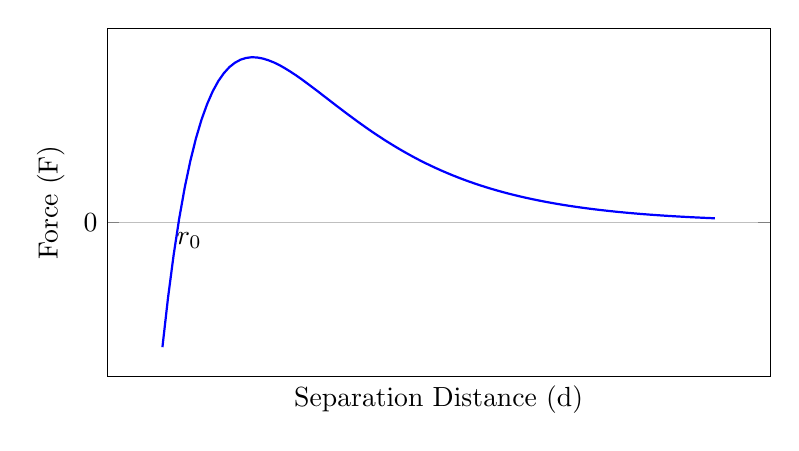
\begin{tikzpicture}
        \begin{axis}[
            xlabel={Separation Distance (d)},
            ylabel={Force (F)},
            grid=major,
            width=10cm,
            height=6cm,
            domain=-0.3:10,
            samples=100,
            xtick = \empty,
            ytick = {0}
        ]
        \addplot[blue, thick] {exp(-x/2) - exp(-x)};
        \node at (axis cs:0.2,0) [anchor=north] {$r_0$};
        
    \end{axis}
    \end{tikzpicture}
    \caption{Force-Separation Curve (Lennard-Jones Force)}
    \label{fig:force-separation}
\end{figure}
\begin{equation}
    E \propto \frac{dF}{dr} \Bigg|_{r_0}
\end{equation}
\begin{definition}[Equilibrium interatomic seperation distance]
The equilibrium interatomic seperation distance, $r_0$, is the distance between two atoms at which the interatomic force is zero. This is due to the interatomic forces being the sum of attractive and repulsive forces.
\end{definition}
\paragraph{Elastic Modulus} Thus, strongly bonded materials have a higher elastic modulus and the slope of the force-seperation curve is steeper at $r_0$.
\subsection{Understanding Other Properties in terms of Atomic Configuration}
\paragraph{Potential Energy-Separation Curve} The potential energy-seperation curve is a plot of the potential energy between two atoms as a function of the distance between them. The potential energy is the area under the force-seperation curve.
\paragraph{Depth of the Minimum Energy Well} The depth of the minimum energy well, $E_0$, is the energy required to break the bond between two atoms. This is the energy required to move the atoms from the equilibrium position to infinity. It is proportional to the melting temperature of the material.
\begin{figure}[h]
    \centering
    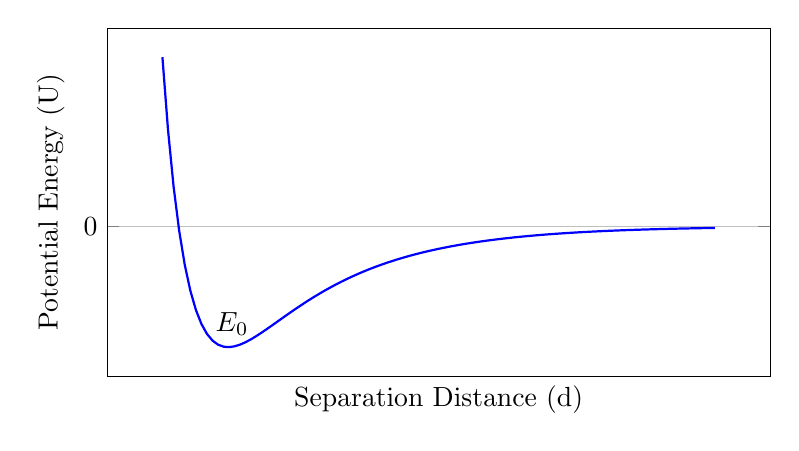
\begin{tikzpicture}
        \begin{axis}[
            xlabel={Separation Distance (d)},
            ylabel={Potential Energy (U)},
            grid=major,
            width=10cm,
            height=6cm,
            domain=-0.3:10,
            samples=100,
            xtick = \empty,
            ytick = {0}
        ]
        \addplot[blue, thick] {-exp(-x/2) + exp(-x)^2};
        \node at (axis cs:1,-0.3) [anchor=north] {$E_0$};
        
    \end{axis}
    \end{tikzpicture}
    \caption{Potential Energy-Separation Curve}
    \label{fig:potential-energy}
\end{figure}
\paragraph{Coefficient of Thermal Expansion} The coefficient of thermal expansion, $\alpha$, is the fractional change in length per degree change in temperature. 
\paragraph{Depth of Potential Energy Curve} The deeper the potential energy curve, the higher the melting temperature and more symetric the curve near $E_0$. This would give the follwoing three properties:
\begin{enumerate}
    \item \textbf{Higher Melting Temperature} The higher the melting temperature, the deeper the potential energy curve.
    \item \textbf{Higher Elastic Modulus} The steeper the slope of the force-seperation curve at $r_0$, the higher the elastic modulus.
    \item \textbf{Lower Coefficient of Thermal Expansion} The more symetric the potential energy curve near $E_0$, the lower the coefficient of thermal expansion.
\end{enumerate}
\subsection{Shear and Tensile Stress}
\subsubsection{Shear}
\paragraph{Shear Stress} Shear stress is the force per unit area acting parallel to the surface. It is given by:
\begin{equation}
    \tau = \frac{F}{A_0}
\end{equation}
\paragraph{Shear Strain} Shear strain is the change in angle between two lines originally perpendicular to each other. It is given by:
\begin{equation}
    \gamma = \frac{\Delta l}{l_0} \approx \tan \theta \approx \theta = \frac{\pi}{2} - \phi
\end{equation}
\paragraph{Shear Modulus} The shear modulus, $G$, is the ratio of shear stress to shear strain. It is given by:
\begin{equation}
    \tau = G \gamma
\end{equation}
\paragraph{Relationship between Shear and Tensile Modulus} The shear modulus is related to the tensile modulus by the following equation:
\begin{equation}
    G = \frac{E}{2(1+\nu)}
\end{equation}
where $\nu$ is the Poisson's ratio.
\paragraph{Poisson's Ratio} Poisson's ratio, $\nu$, is the ratio of lateral strain to axial strain. It is given by:
\begin{equation}
    \nu = -\frac{\epsilon_{\text{lat}}}{\epsilon_{\text{axial}}}
\end{equation}
\subsection{Testing}
\begin{definition}[Gauge Length]
The gauge length, $l_0$, is the length of the sample over which the strain is measured.
\end{definition}
\begin{definition}[Reduced Section]
The reduced section is the part of the sample where the cross-sectional area is reduced to a smaller value.
\end{definition}
\paragraph{} Gauge length is always no longer than the reduced section. The reduced section is where the sample will likely break.
\paragraph{Testing Ceremics} In relation to tensile testing, ceramics have the following properties:
\begin{itemize}
    \item \textbf{Brittle} Ceramics are brittle and will break suddenly.
    \item \textbf{High Strength} Ceramics have high strength and thus difficult to machine the sample.
    \item \textbf{Sample Alignment} The sample must be aligned properly to test for pure tension. Unlike metals and polymers, which are self-aligning.
    \item \textbf{Fracture} Ceramics will fracture while still off-axis. Hence, there would be a large shear component. 
\end{itemize}
\paragraph{} Thus, we often approxiate tensile behaviour with a point loading on a horizontal beam, with two point support (3 point bending test). Peak stress is given by:
\begin{equation}
    \sigma_{\text{peak}} = \frac{3FL}{2bd^2}
\end{equation}
, where:
\begin{itemize}
    \item $L$ (span) is the distance between the two supports.
    \item $b$ is the width of the sample
    \item $d$ is the thickness/depth of the sample
\end{itemize}
\section{Seleection of Materials}
\subsection{Material Performance}
\begin{example}[Aircraft Wing Spar]
    The aircraft wing spar is beam (loaded in bending) that supports the wing. The spar is made of a material with the objective of minimize mass under the following constraints:
    \begin{itemize}
        \item \textbf{Deflection} There is a maximum allowable deflection of the wing.
        \item There is more..., but for this example, we will only consider the deflection.
    \end{itemize}
    The material selection solve for a \textbf{light stiff beam}.

    \paragraph{Mass} The mass of the beam is given by:
    $$ m = \rho V = \rho A L $$
    \paragraph{Deflection} The deflection of the beam is given by:
    \begin{equation}
        \delta = \frac{FL^3}{48EI} 
    \end{equation}
    \begin{align*} 
        \intertext{For a beam with a rectangular cross-section, we have:}
        \delta &= \frac{FL^3}{48E} \cdot \frac{12}{bh^3} = \frac{FL^3}{4Ebh^3}  
        \intertext{We can set $b$ proportional to $h$:}
        \delta &= \frac{FL^3}{cE} \cdot \frac{1}{A^2},\quad \text{for some constant $c$} 
        \intertext{We can then isolate for $A$, the free variable, and minimize the mass via the objective equation $m = \rho A L$:}
        A &= \sqrt{\frac{FL^3}{cE\delta}} \\
        m &= \rho L \sqrt{\frac{FL^3}{cE\delta}} = \rho L \sqrt{\frac{FL^3}{cE\delta}}
        \intertext{Arrange into the form (functional)(geometric)(material):}
        m &= \left(\frac{F}{c\delta}\right)^\frac{1}{2} \cdot \left(L^\frac{5}{2}\right)\cdot\left(\frac{\rho}{E^\frac{1}{2}}\right)
    \end{align*}
\end{example}
\paragraph{Material Peformance Index} The material performance index is given by:
    \begin{equation}
        \text{Material Performance Index (MSI)} = \frac{E^\frac{1}{2}}{\rho}
\end{equation}
\paragraph{MPI Graph} We plot $\log E$ against $\log \rho$ to get the MPI graph. 
\paragraph{Tempered Glass} Temperglass are made to resist tension. It is done by applying a compressive stress to the surface of the glass. This is done by cooling the surface of the glass faster than the core or chemically treating the surface.
\subsection{Density}
\paragraph{Density} The density of a material is given by:
\begin{equation}
    \rho = \frac{m}{V}
\end{equation}
\paragraph{Archimedes' Principle} The buoyant force on an object is equal to the weight of the fluid displaced by the object. Derive from that, we have:
\begin{equation}
    \rho = \frac{m}{V} = \frac{m_{\text{object}}}{m_{\text{object}} - m_{\text{object in fluid}}}
\end{equation}
\section{Atomic Structures}
\subsection{General Definitions}
\paragraph{Ordered structures} We have the following three orders:
\begin{enumerate}
    \item \textbf{Long Range Order (LRO)} Atoms are arranged in a well-defined pattern over long distances in repeating units. \\
    (Example) Diamonds, some polymers, most metals, many ceramics, graphite, quartz, etc.
    \item \textbf{Short Range Order (SRO)} Periodic arrangement of atoms over a few atomic or molecular spacings. \\
    (Example) Most polymers, glasses, amorphous materials, etc.
    \item \textbf{No Order (NO)} Atoms are randomly arranged. \\
    (Example) Ideal gases, etc.
\end{enumerate}
\paragraph{Describing Crystal Structures} We can describe crystal structures by the following:
\begin{itemize}
    \item \textbf{Unit Cell} The smallest repeating unit of a crystal structure that could be used to represent the entire crystal.
    \item \textbf{Lattice} The repeating arrangement of points that repersent the positions of atoms in the unit cell.\\
    (Example) Simple Cubic, Body-Centered Cubic, Face-Centered Cubic, etc.
    \item \textbf{Lattice Plus Basis} \textit{Not required for this course}
\end{itemize}
\paragraph{Theortical Density of Metals} The theoretical density of metals is given by:
\begin{equation} \label{eq:theoretical-density}
    \rho = \frac{nM}{V_c N_A}
\end{equation}
, where:
\begin{itemize}
    \item $n$ is the number of atoms in the unit cell.
    \item $M$ is the atomic mass of the element (amu = g/mol).
    \item $V_c$ is the volume of the unit cell.
    \item $N_A$ is Avogadro's number ($6.022 \times 10^{23} \text{mol}^{-1}$)
\end{itemize}
\subsection{Describing Basic Unit Cells}
\begin{definition}[Coordination Number (CN)]
    The coordination number is the number of nearest neighbors an atom has in a crystal structure.
\end{definition}
\begin{definition}[Atomic Packing Factor (APF)]
    The atomic packing factor is the fraction of the volume of the unit cell that is occupied by hard spheres. It is given by:
    \begin{equation}
        \text{APF} = \frac{\text{Volume of atoms in unit cell}}{\text{Volume of unit cell}}
    \end{equation}
\end{definition}
\paragraph{Simple Cubic (SC)} The simple cubic structure has the following properties:
\begin{itemize}
    \item \textbf{Centers of atoms} Located at the eight corners of a cube
    \item \textbf{Rare Packing Density}  Due to low packing density (only known example: Polonium, Po)
    \item \textbf{Close-packed directions} As cube edges.
    \item \textbf{Coordination Number} Number of nearest neighbor: 6
\end{itemize}
\paragraph{Face-Centered Cubic (FCC)} The face-centered cubic structure has an atom on the centre of each face of the cube. It has the following properties:
\begin{itemize}
    \item \textbf{Ductile} and \textbf{Malleable} due to the close-packed planes. Common examples include: \\ $\ch{Al}\, ,\ch{Cu}\, ,\ch{Au}\, ,\ch{Ag}$.
    \item \textbf{Coordination Number} Number of nearest neighbor: 12
    \item \textbf{Close-packed directions} As cube diagonals.
    \item \textbf{Theortical Density} The theoretical density of FCC is derived from Equation (\ref{eq:theoretical-density}):
    \begin{align}
        \rho &= \frac{nM}{V_c N_A} \nonumber \\
        \intertext{With $n = 4$ (8 corners $\times \frac{1}{8}$ atom each + 6 faces $\times \frac{1}{2}$ atom each) and $V_c = a^3$ (where $a$ is the \textbf{lattice parameter}):}
        \rho_\text{FCC} &= \frac{4M}{a^3 N_A} \nonumber \\
        \intertext{We can then obtain $a$ via the relationship between the atomic radius, $r$, and the lattice parameter via the geometry on the close-packed direction (face diagonal):}
        a &= 2\sqrt{2}r \nonumber \\
        \intertext{Substitute $a$ back into the equation:}
        \rho_\text{FCC} &= \frac{4M}{(2\sqrt{2}r)^3 N_A} = \frac{4M}{16\sqrt{2}r^3 N_A} \nonumber \\
        &= \frac{M}{4\sqrt{2}r^3 N_A} 
    \end{align}
    \item \textbf{Atomic Packing Factor} The atomic packing factor of FCC is given by:
    \begin{equation}
        \text{APF}_\text{FCC} = \frac{\text{Volume of atoms in unit cell}}{\text{Volume of unit cell} } = \frac{4 \times \frac{4}{3}\pi r^3}{a^3} = \frac{4 \times \frac{4}{3}\pi r^3}{(2\sqrt{2}r)^3} = \frac{\pi}{6\sqrt{2}} = \textbf{0.74}
    \end{equation}
    This is the highest possible packing factor for spheres. Thus, no other structure can have a higher packing factor.
    \item \textbf{Stacking} The FCC structure can be thought of as stacking close-packed planes. The stacking sequence is ABCABC... (where A, B, and C describe the orientation hexagonal close-packed planes).
\end{itemize}
\paragraph{Hexagonal Close-Packed (HCP)} The hexagonal close-packed structure is \textbf{crytal structure} by stacking close-packed hexagonal planes. It has the following properties:
\begin{itemize}
    \item \textbf{Coordination Number} Number of nearest neighbor: 12
    \item \textbf{Close-packed directions} As cube diagonals.
    \item \textbf{Theortical Density} The theoretical density of HCP is derived from Equation (\ref{eq:theoretical-density}):
    \begin{align}
        \rho &= \frac{nM}{V_c N_A} \nonumber \\
        \intertext{With $n = 6$ (12 corners $\times \frac{1}{6}$ atom each) and $V_c = a^3$:}
        \rho_\text{HCP} &= \frac{6M}{a^3 N_A} 
    \end{align}
    \item \textbf{Atomic Packing Factor} The atomic packing factor of HCP is given by:
    \begin{equation}
        \text{APF}_\text{HCP} = \frac{\text{Volume of atoms in unit cell}}{\text{Volume of unit cell} } = \frac{6 \times \frac{4}{3}\pi r^3}{a^3} = \frac{6 \times \frac{4}{3}\pi r^3}{a^3} = \textbf{0.74}
    \end{equation}
    \item \textbf{Stacking} The HCP structure can be thought of as stacking close-packed planes. The stacking sequence is ABAB...
\end{itemize}
\begin{example}[Density of Aluminum]
    Given that the atomic radius of aluminum is $r = 143$ pm and the atomic mass is $M = 26.98$ g/mol, we can calculate the density of aluminum with FCC structure. We have:
    \begin{align*}
        \rho_\text{Al} &= \frac{M}{4\sqrt{2}r^3 N_A} = \frac{26.98}{4\sqrt{2} \times (143 \times 10^{-12})^3 \times 6.022 \times 10^{23}} \\
        &= \frac{26.98}{4\sqrt{2} \times (143 \times 10^{-12})^3 \times 6.022 \times 10^{23}} = 2.7 \text{ g/cm}^3
    \end{align*}
\end{example}
\paragraph{Body-Centered Cubic (BCC)} The body-centered cubic structure has an atom at the centre of the cube. It has the following properties:
\begin{enumerate}
    \item \textbf{Coordination Number} Number of nearest neighbor: 8
    \item \textbf{Atomic Packing Factor} The atomic packing factor of BCC is given by:
    \begin{equation}
        \text{APF}_\text{BCC} = \frac{\text{Volume of atoms in unit cell}}{\text{Volume of unit cell} } = \frac{2 \times \frac{4}{3}\pi r^3}{a^3} = \frac{2 \times \frac{4}{3}\pi r^3}{(4r/\sqrt{3})^3} = \textbf{0.68}
    \end{equation}
    \item \textbf{Close Packed Directions} As cube diagonals.
    \item \textbf{Theortical Density} The theoretical density of BCC is derived from Equation (\ref{eq:theoretical-density}):
    \begin{align}
        \rho &= \frac{nM}{V_c N_A} \nonumber \\
        \intertext{With $n = 2$ (8 corners $\times \frac{1}{8}$ atom each + 1 center atom) and $V_c = a^3$:}
        \rho_\text{BCC} &= \frac{2M}{a^3 N_A} 
    \end{align}
    \item \textbf{Stacking} The BCC structure can be thought of as stacking close-packed planes. The stacking sequence is ABAB...
\end{enumerate}
\section{Geometric Properties of Crystals}
\subsection{Crystallographic Directions and Planes}
\paragraph{Point Coordinates} A lattice positon in a unit cell is determined as fractional multiples of the unit cell edge lengths $a$, $b$, and $c$. (Defining the origin at one corner of the unit cell and $a=b=c=\textbf{1}$)
\paragraph{Crystallographic Directions} A crystallographic direction is a line between two points in a crystal. It is denoted by square brackets, $[uvw]$. The direction is determined from the ``tail'' to the ``head'' of the vector. Also:
\begin{enumerate}
    \item It \textbf{shall not} include commas; and
    \item It \textbf{shall be reduced}to the smallest integers; and
    \item Negative signs are represented by a bar over the number.
\end{enumerate}
\begin{example}
    The crystallographic direction from $(0,0,0)$ to $(-1,0,1/2)$ is $[\bar{2}01]$.
\end{example}
\paragraph{Family of Directions} A family of directions is a set of directions that are parallel to each other. It is denoted by $<uvw>$.
\begin{example}
    The family of directions $<100>$ is the set of directions $[100]$, $[010]$, $[001]$, $[\bar{1}00]$, $[0\bar{1}0]$, and $[00\bar{1}]$.
\end{example}
\paragraph{Angle between Directions} The angle between two directions in a \textbf{cubic} crystal is given by:
\begin{equation}
    \cos \theta = \frac{h_1h_2 + k_1k_2 + l_1l_2}{\sqrt{h_1^2 + k_1^2 + l_1^2}\sqrt{h_2^2 + k_2^2 + l_2^2}}
\end{equation}
, which is simply the normalized dot product of the two vectors.
\paragraph{Crystallographic Planes} A crystallographic plane is a set of parallel planes in a crystal. It is denoted by $(hkl)$. The plane is determined by the intercepts on the $x$, $y$, and $z$ axes. 
\paragraph{} Generally, we find the intercepts by finding the points where the plane intersects the axes. We then take the reciprocals of the intercepts and multiply by the smallest integer to get the Miller Indices.
\paragraph{Family of Planes} A family of planes is a set of planes that are parallel to each other. It is denoted by $\{hkl\}$.
\paragraph{Distance between Planes} The distance between two planes with miller indices $(h_1k_1l_1)$ and $(h_2k_2l_2)$ is given by:
\begin{equation}
    d = \frac{a}{\sqrt{h^2 + k^2 + l^2}}
\end{equation}
, where $a$ is the lattice parameter.
\subsection{X-Ray Diffraction} The diffraction pattern is used to determine the crystal structure. By measuring the n$^\text{th}$ order peak angle $\theta_c$ and the wavelength of the X-ray, we can determine the distance between planes:
\begin{align}
    2d\sin \theta &= n\lambda \nonumber \\
    d &= \frac{n\lambda}{2\sin \theta_c}
    \intertext{Thus, we could determine the lattice parameter $a$ by the following equation:}
    a &= \frac{n\lambda}{2\sin \theta_c} \sqrt{h^2 + k^2 + l^2}
\end{align}
\subsection{Geometrcally Ideal Crystal Structures}
\paragraph{Coordination Number and Ratio} The coordination number increases with $\frac{r_{\text{cation}}}{r_{\text{anion}}}$ (The ionic radii ratio).  It relates to coordination number as follows:
\begin{table}[h]
    \centering
    \begin{tabular}{|c|c|c|}
        \hline
        \textbf{Ionic Radii Ratio} & \textbf{Coord. Number} & \textbf{Name} \\
        \hline
        $<$ 0.155 & 2 & Linear \\
        0.155 - 0.225 & 3 & Trigonal Planar \\
        0.225 - 0.414 & 4 & Tetrahedral \\
        0.414 - 0.732 & 6 & Octahedral \\
        0.732 - 1.0 & 8 & Cubic \\
        \hline
    \end{tabular}
    \caption{Coordination Number and Ionic Radii}
    \label{tab:coordination-number}
\end{table} 
\begin{definition}[AX Type]
    The AX type is a crystal structure where the cation and anion are of the same ratio. 
\end{definition}
\begin{example}[AX Type: $\ch{NaCl}$ rock salt]
    The $\ch{NaCl}$ structure is an AX type structure. The cation and anion are of the same ratio. Soldium (Cation) has radius $r_{\text{Na}} = 0.102$ nm and Chlorine (Anion) has radius $r_{\text{Cl}} = 0.181$ nm. The ratio is:
    $$ \frac{r_{\text{cation}}}{r_{\text{anion}}} = \frac{0.102}{0.181} = 0.56 $$
    Thus, the coordination number is 6.\\
    Additionally, we could calculate its theoretical density. It has 4 cation and 4 anion in the unit cell. The volume of the unit cell is $a^3$, and it follows a FCC structure. Thus, the density is: 
    \begin{align*}
        \rho &= \frac{4M_{\text{Na}} + 4M_{\text{Cl}}}{a^3 N_A} = \frac{4(22.99) + 4(35.45)}{a^3 N_A} \\
        &= \frac{4(22.99) + 4(35.45)}{(2\sqrt{2}r_{\text{Na}})^3 N_A} = \frac{4(22.99) + 4(35.45)}{(2\sqrt{2} \times 0.102)^3 N_A} \\
        &= \frac{4(22.99) + 4(35.45)}{(2\sqrt{2} \times 0.102)^3 N_A} = 2.16 \text{ g/cm}^3
    \end{align*}
\end{example}
\begin{example}[AX Type: $\ch{ZnS}$, Zinc Blende]
    The $\ch{ZnS}$ structure is an AX type structure. It has a FCC structure with CN = 4. The radius of Zinc (Cation) is $r_{\text{Zn}} = 0.074$ nm and the radius of Sulfur (Anion) is $r_{\text{S}} = 0.184$ nm. The ratio is:
    $$ \frac{r_{\text{cation}}}{r_{\text{anion}}} = \frac{0.074}{0.184} = 0.40 $$
\end{example}
\begin{example}[AX$_2$ Type: $\ch{CaF2}$]
    The $\ch{CaF2}$ structure is an AX$_2$ type structure. It has a FCC structure with CN = 8. The radius of Calcium (Cation) is $r_{\text{Ca}} = 0.099$ nm and the radius of Fluorine (Anion) is $r_{\text{F}} = 0.133$ nm. The ratio is:
    $$ \frac{r_{\text{cation}}}{r_{\text{anion}}} = \frac{0.099}{0.133} = 0.74 $$
\end{example}
\section{Stress-Strain Behavior}
\paragraph{Uniformly Distributed Elongation} The elongation of a material is uniformly distributed within the gauge length. The initial values, referred to as the ``elastic region," are characterized as uniformly elastic. 
\paragraph{Non-Linear Elastic} There is also a non-linear region where the material remains elastic but is not uniformly distributed.
\paragraph{Localized Plastic Deformation} The material then enters the plastic region where the deformation is localized. The material is permanently deformed. This is characterized by the ultimate tensile strength (this is bad when it happens).
\paragraph{Necking} The material then necks, where the cross-sectional area decreases. The material is then strained until it breaks.
\paragraph{True Stress} The true stress is given by:
\begin{equation}
    \sigma_T = \frac{F}{A_i}
\end{equation}
, where $A_i$ is the instantaneous cross-sectional area.
\paragraph{Ultimate Tensile Strength} The ultimate tensile strength is the maximum stress on the stress-strain curve.
\paragraph{Strengthening} Plastic deformation is made more difficult by the following mechanisms:
\begin{enumerate}
    \item \textbf{Strain Hardening} Preloading beyond the elastic region - upon plastic deformation, the material will have a higher yield strength.
    \item \textbf{For Metals and Alloys} The following mechanisms are used:
\end{enumerate}
\paragraph{Strain Hardening Equation} The true stress-strain curve can be emprically described by the following equation:
\begin{equation}
    \sigma_T = K \epsilon^n_T
\end{equation}
, where $K$ is the Strain Hardening coefficient and $n$ is the strain hardening exponent. Both of these values are material properties.
\paragraph{True Strain} Since $\epsilon_i = \frac{\Delta l_i}{l_0 + \Delta l_{i-1}}$ we can compute a Rieman sum to get the true strain:
\begin{equation}
    \epsilon_T = \int^{l_f}_{l_0} \frac{dl}{l} = \ln \left(\frac{l_f}{l_0}\right)
\end{equation}
\paragraph{Strain Rate} The strain rate is the rate at which the material is deformed. It is given by:
\paragraph{} But, before necking, we can assume $V_0 = V_i$ and $A_i = \frac{A_0 l_0}{l_i}$. Thus, we have:
\begin{align}
    \sigma_T &= \frac{F}{A_i} = \frac{F}{\frac{A_0 l_0}{l_i}} = \frac{F l_i}{A_0 l_0} = \frac{F}{A_0} \cdot \frac{l_i}{l_0} = \sigma \cdot \frac{l_i}{l_0}  \nonumber \\
    &= \sigma \cdot (1 + \epsilon)
    \intertext{and,}
    \epsilon_T &= \ln \left(1 + \epsilon\right)
\end{align}
\subsection{Imperfections}
\paragraph{Dislocation} Recal that plastic deformation occurs by step-wise breaking of atomic bonds. This is done by the movement of dislocations. \textbf{Strengthening mechanisms in Metals} rely on inhibiting the movement of dislocations.
\begin{definition}[Dislocation]
    A dislocation is the breaking and reforming of bonds, one row at a time. It is a line defect in the crystal structure.
\end{definition}
\paragraph{Crystalline Imperfections} We use crystalline imperfections to inhibit the movement of dislocations. These imperfections include:
\begin{itemize}
    \item \textbf{Point Imperfections (Defects)} Vacancies, interstitials, and substitutional atoms.
    (Example) Solid solution strengthening.
    \item \textbf{Line Imperfections} Dislocations.
    \item \textbf{Area Imperfections} Grain boundaries of the interface between two grains and free surfaces.
    \item \textbf{Volume Imperfections} Second phase particles.
\end{itemize}
\paragraph{Solid Solution Strengthening} [Alloying] The addition of a solute to a solvent to inhibit the movement of dislocations. There is two types:
\begin{enumerate}
    \item \textbf{Interstitial Impurities} The solute atoms are smaller than the solvent atoms. This the impurites to be in the interstitial sites.
    \item \textbf{Substitutional Impurities} The solute atoms are larger than or as large as the solvent atoms ($<10 \% \Delta \varnothing$, similar electornegativity.). This causes the impurities substitute the lattice sites.
\end{enumerate}
\paragraph{Vacancies} Vacancies are missing atoms in the lattice. They are created by thermal vibrations. They are used to inhibit the movement of dislocations.
It slightly nudges nearby atoms, creating \textbf{lattice strain} that make it harder for dislocations to move.
\paragraph{Machaism - Diffusion of Impurities} In positve edge dislcation, it has compession above disvlation line, and tension below. The impurities will `pin' the dislocation, making it harder to move.
\paragraph{Plastic Deformation} We can also strengthen the material by increasing the number of dislocations. This is done by plastic deformation methods:
\begin{enumerate}
    \item Cold Work
    \item Forging/Strain Hardening
\end{enumerate}
\paragraph{Mechanisms of Strengthening} Plastic deformation increases number of dislocations, which inhibits one another due to the strain fields.
\begin{definition}[Grain Boundaries]
    Grain boundaries are the interface between two grains. Grains are regions of the same crystal structure but with different orientations.
\end{definition}
\paragraph{Grain Size Reduction} Dislcations tend to move in the direction of the grain boundry (GB). Thus, reducing the grain size reduces the distance the dislocation can move. In addition, there are atomic strain due to the difference of bond lenght between grains, contributing to the strain field. It is given by:
\begin{equation}
    \sigma = \sigma_0 + \frac{K_y}{d}
\end{equation}
\paragraph{Second Phase Particles} Second phase particles are particles of a different phase in the material. They can be used to inhibit the movement of dislocations. They are often hard, brittke phases.
\paragraph{Dislcations (Slips)} Occurs on the plane with the highest planar density. The slip direction is the direction with the highest linear density. The slip system is the combination of the slip plane and slip direction.
\paragraph{} FCC has 4 unique planes, each with 3 unique directions. Thus, there are 12 unique slip systems. Compare this to HCP, which has only base plane.
\paragraph{Resolved Stear Stress} Consider single crystal with a certain plane. Let $\phi$ be the angle between the normal of the plane and the direction of the applied stress, and $\lambda$ be the angle between the plane and the orthonal of the applied stress. The resolved shear stress is given by:
\begin{equation}
    \tau = \sigma \cos \phi \cos \lambda
\end{equation}
\paragraph{Critcal Resolved Shear Stress} The critical resolved shear stress is the minimum shear stress required to move a dislocation. When the resolved shear stress equal the critical resolved shear stress, the dislocation will move, and:
\begin{equation}
    \sigma = \sigma_{y}
\end{equation}
So,
\begin{equation}
   \tau_{\text{CRSS}} = \sigma_{y} \cos \phi \cos \lambda
\end{equation}
\paragraph{Note} Most crystals are polycrystalline, so dislocation must be able to move to the neibouring crystal.
\paragraph{Burgers Vector} The Burgers vector is the vector that describes the dislocation. It is the vector that closes the loop of the dislocation. It is given by:
\begin{equation}
    \vec{b} = \vec{b}_1 + \vec{b}_2
\end{equation}
\section{Polymers} 
\paragraph{Polymer} Polymers could be britte or elastic (elastomers). They are made of long chains of monomers. Interestingly, polymers have necking points lower than its ultimate tensile strength.
\begin{center}
    \textit{``Why does polymers continue to stretch after necking?''}
\end{center}
\paragraph{Polymer Structure} Polymers are made of long chains of monomers. The chains are held together by weak van der Waals forces. The chains are entangled.
\\ (Example) Polyethylene are made of long chains of carbon atoms with two hydrogen atoms attached to each carbon atom.
\paragraph{Ans: (Chain-Oriented)} The chains are originally entangled. When the polymer is stretched, the chains are straightened to align with the load. More of the load is taken by the covalent bonds, which are stronger than the van der Waals forces. This serves as an important strengthening mechanism.
\paragraph{Note} In a polymer, the elastic response is from numerrous bond types.
\paragraph{Crylistallinity} Polymers cannot be 100\% crystalline. A polymer could be semi-crystalline, where the polymer has both crystalline and amorphous regions. Since the crystalline regions are stronger, increasing the crystallinity is a important strengthening mechanism.
\begin{enumerate}
    \item \textbf{Tmerpeature} Increasing the crtystallinity permits the polymer have higher service temperature. 
    \item \textbf{Chemical Resistance} Crystalline regions are more resistant to chemcial dissolution.
\end{enumerate}
\paragraph{Different Mer Units} Different mer units have different properties. Listed below are some common mer units:
\begin{itemize}
    \item \textbf{Polyethylene} (PE) - Made of long chains of carbon atoms with two hydrogen atoms attached to each carbon atom.
    \item \textbf{Polypropylene} (PP) - Similar to PE, but with a methyl group attached to the carbon atom.
    \item \textbf{Polyvinyl Chloride} (PVC) - Made of long chains of carbon atoms with a chlorine atom attached to each carbon atom. Chlorine are more electronegative than carbon, so the bond is polar and form stornger van der Waals forces.
    \item \textbf{Polystyrene} (PS) - Made of long chains of carbon atoms with a phenyl group attached to each carbon atom.
    \item \textbf{Polytetrafluoroethylene} (PTFE) - Made of long chains of carbon atoms with two fluorine atoms attached to each carbon atom. The florine is to protect the carbon backbone. Hoowever, it is mechanically weak as the dipole moment is low.
    \item \textbf{Polymethyl Methacrylate} (PMMA) - Made of long chains of carbon atoms with a methyl group and a methacrylate ($-\ch{OC(=O)}$) group attached to each carbon atom. It is opticall tranparnet the methacrylate group prevent crtystallinity, hence amorphous and no crystal boundaries.
\end{itemize}
\subsection{Viscoelasitcity and Thermal Properties}
\paragraph{Viscoelasticity} Polymers are viscoelastic. They have both viscous and elastic properties. The viscous properties are due to the entanglement of the chains. The elastic properties are due to the covalent bonds.
\paragraph{Time-Dependent Behavior} For a given stress/strain, the strain/stress will decrease with time. This is due to the viscous properties of the polymer.
\paragraph{Relaxation Modulus} The relaxation modulus is the modulus of the polymer as a function of time. It is given by:
\begin{equation}
    E(t) = \frac{\sigma(t)}{\epsilon_0}
\end{equation}
The relaxation modulus is also relate to the temperature of the polymer. The relaxation modulus decreases with temperature.
\paragraph{Glassy Transition} The glassy transition is the temperature at which the polymer changes from a glassy state to a rubbery state. The glassy state is characterized by a high modulus and low strain. The rubbery state is characterized by a low modulus and high strain. The temperature is denoted as $T_g$.
This is due to the temperature overcoming the intermolecular forces of the amorphous reigions, but the crystalline regions are still intact as the van der Waals foce is stronger.
\paragraph{Melting} THe melting temperature is the temperature at which the polyme the intermolecular forces of the crystalline regions are overcome. The polymer then melts as chains slide past each other. 
\paragraph{Thermosat} Thermosat are polymers that do not melt. They are made of cross-linked chains or network polymers. The cross-links prevent the chains from sliding past each other. Elastomers are typically thermosets.
\subsection{Optical Properties}
\paragraph{PMMA} PMMA is a transparent polymer. It is used in optical applications. The transparency is due to the lack of \textbf{scattering events}.
\begin{definition}[Scatter Event]
    A scatter event is an event that causes light to be scattered. It is due to the difference in refractive index between the polymer and the air.
\end{definition}
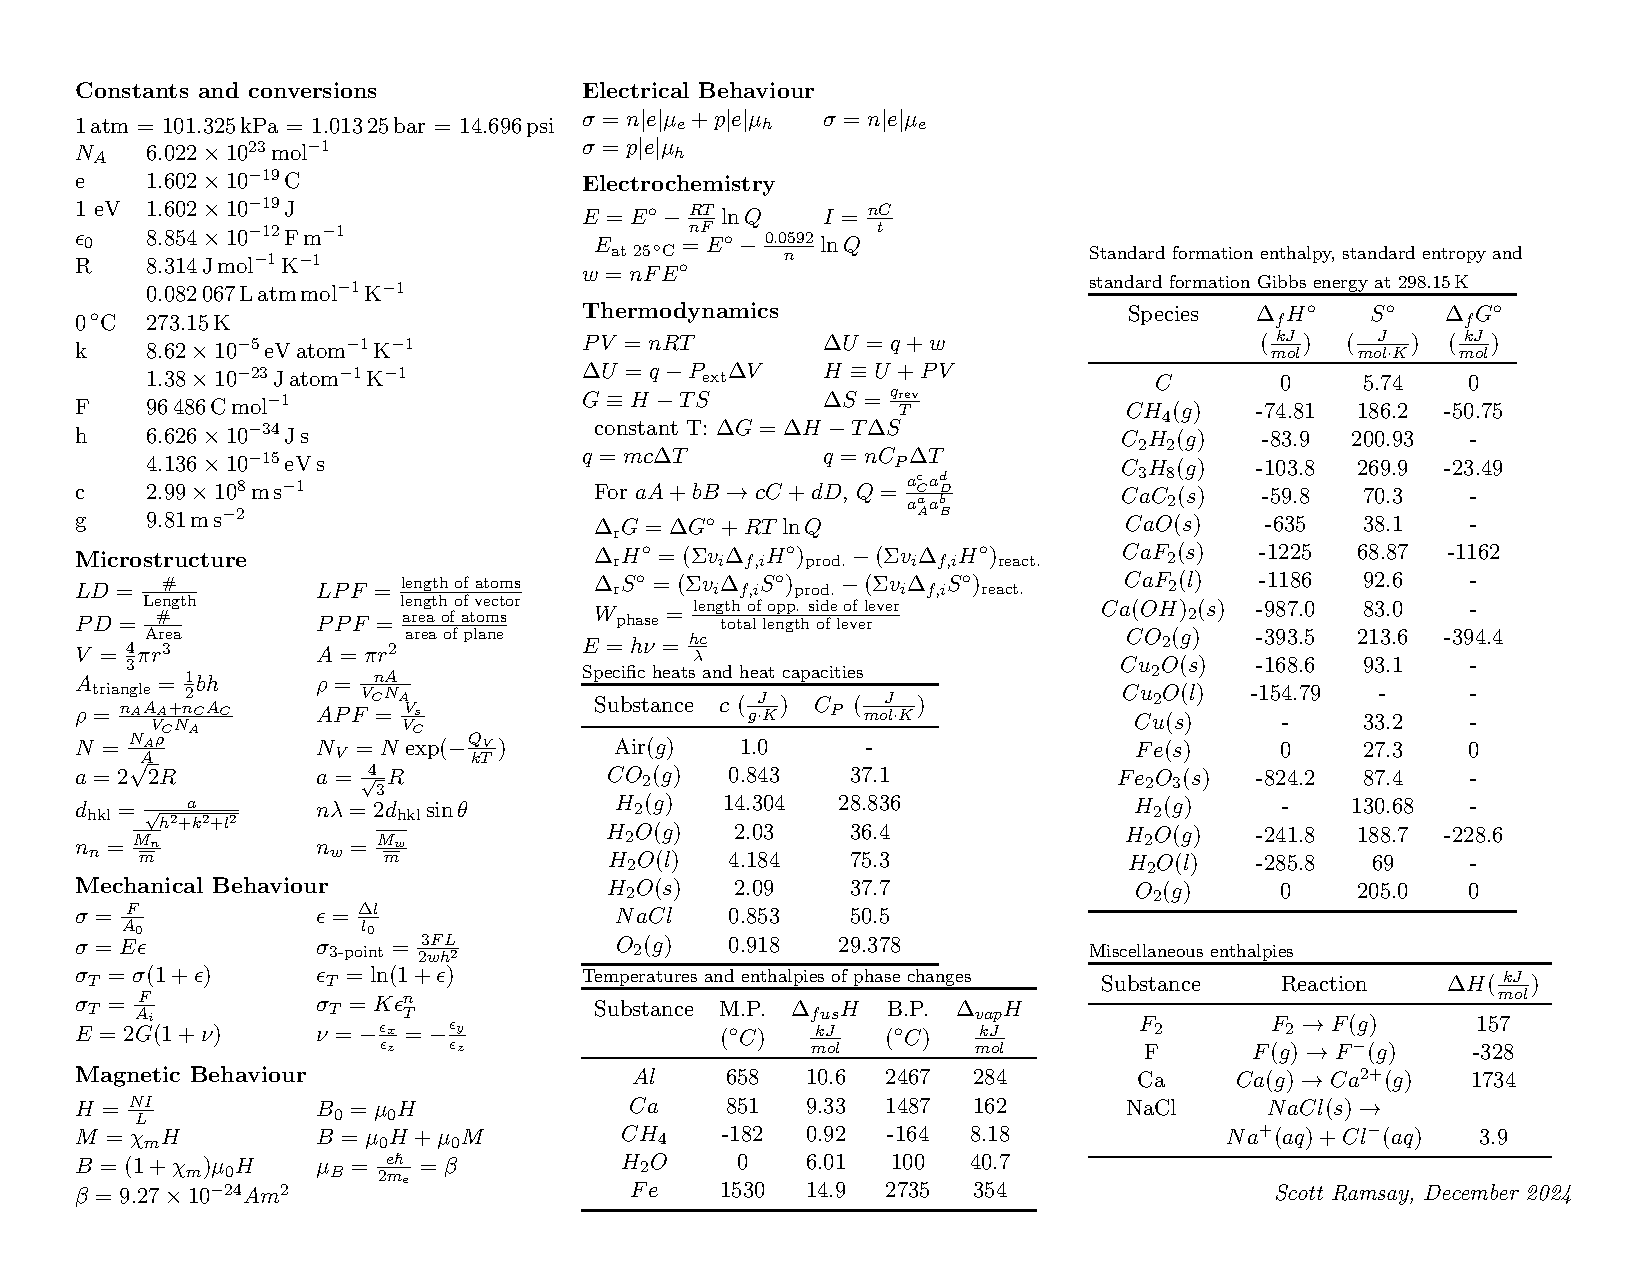
\includepdf[pages=-, angle=90]{EquationSheet.pdf}

\end{document}
